\documentclass[answers,12pt,addpoints]{exam}
\usepackage{import}

\import{C:/Users/prana/OneDrive/Desktop/MathNotes}{style.tex}

% Header
\newcommand{\name}{Pranav Tikkawar}
\newcommand{\course}{01:640:495}
\newcommand{\assignment}{Lecture 1}
\author{\name}
\title{\course \ - \assignment}

\begin{document}
\maketitle


\newpage
\section*{Lecture 1}
\begin{questions}
    \question Given 3 (non colinear) points $A, B, C$ in the plane, Find a quadratic polynomial $f(x)$ passes through all three points.\\
    Define $A = (x_1, y_1), B = (x_2, y_2), C = (x_3, y_3)$
    \begin{solution}
        Given these three points, we can write the following equations:
        \begin{align*}
            f(x_1) &= y_1\\
            f(x_2) &= y_2\\
            f(x_3) &= y_3
        \end{align*}
        where $f(x) = ax^2 + bx + c$. Substituting the values of $x_1, x_2, x_3$ in the above equations, we get:
        \begin{align*}
            ax_1^2 + bx_1 + c &= y_1\\
            ax_2^2 + bx_2 + c &= y_2\\
            ax_3^2 + bx_3 + c &= y_3
        \end{align*}
        we solve this system by solving the following matrix equation:
        \begin{align*}
            \begin{bmatrix}
                x_1^2 & x_1 & 1\\
                x_2^2 & x_2 & 1\\
                x_3^2 & x_3 & 1
            \end{bmatrix}
            \begin{bmatrix}
                a\\
                b\\
                c
            \end{bmatrix}
            &=
            \begin{bmatrix}
                y_1\\
                y_2\\
                y_3
            \end{bmatrix}
        \end{align*}
        Clearly the matrix is invertible since the points are non-colinear. Thus, we can solve for $a, b, c$ and get the quadratic polynomial $f(x)$.
        \begin{align*}
            \begin{bmatrix}
                a\\
                b\\
                c
            \end{bmatrix} = 
            \begin{bmatrix}
                x_1^2 & x_1 & 1\\
                x_2^2 & x_2 & 1\\
                x_3^2 & x_3 & 1
            \end{bmatrix}^{-1}
            \begin{bmatrix}
                y_1\\
                y_2\\
                y_3
            \end{bmatrix}
        \end{align*}
        Replacing the values of $a, b, c$ in $f(x)$, we get the required quadratic polynomial.\\\\
        We can similarly motivate this by choosing the expression in a way that is aligned w/ the data :
        \begin{align*}
            f(x) = \theta_1 (x - x_2)(x - x_3) + \theta_2 (x - x_1)(x - x_3) + \theta_3 (x - x_1)(x - x_2)
        \end{align*}
        Thus our goal is to find $\theta_1, \theta_2, \theta_3$ such that $f(x_1) = y_1, f(x_2) = y_2, f(x_3) = y_3$. Substituting the values of $x_1, x_2, x_3$ in the above equation, we get:
        \begin{align*}
            \theta_1 (x_1 - x_2)(x_1 - x_3) &= y_1\\
            \theta_2 (x_2 - x_1)(x_2 - x_3) &= y_2\\
            \theta_3 (x_3 - x_1)(x_3 - x_2) &= y_3
        \end{align*}
        We can solve this system by solving the following matrix equation:
        \begin{align*}
            \begin{bmatrix}
                (x_1 - x_2)(x_1 - x_3) & 0 & 0\\
                0 & (x_2 - x_1)(x_2 - x_3) & 0\\
                0 & 0 & (x_3 - x_1)(x_3 - x_2)
            \end{bmatrix}
            \begin{bmatrix}
                \theta_1\\
                \theta_2\\
                \theta_3
            \end{bmatrix}
            &=
            \begin{bmatrix}
                y_1\\
                y_2\\
                y_3
            \end{bmatrix}
        \end{align*}
        Clearly the matrix is invertible and the solution given by:
        \begin{align*}
            \begin{bmatrix}
                \theta_1\\
                \theta_2\\
                \theta_3
            \end{bmatrix} = 
            \begin{bmatrix}
                (x_1 - x_2)(x_1 - x_3) & 0 & 0\\
                0 & (x_2 - x_1)(x_2 - x_3) & 0\\
                0 & 0 & (x_3 - x_1)(x_3 - x_2)
            \end{bmatrix}^{-1}
            \begin{bmatrix}
                y_1\\
                y_2\\
                y_3
            \end{bmatrix}\\
        \end{align*}
        \begin{align*}
            \theta_1 = \frac{y_1}{(x_1 - x_2)(x_1 - x_3)}\\
            \theta_2 = \frac{y_2}{(x_2 - x_1)(x_2 - x_3)}\\
            \theta_3 = \frac{y_3}{(x_3 - x_1)(x_3 - x_2)}
        \end{align*}
    \end{solution}    
\end{questions}
\section*{Lecture 2}
\textbf{Set} is the most important mathematical object.\\
We then use \textbf{functions} to map between sets.\\
\textbf{Injections} are functions that map distinct elements to distinct elements. AKA one-to-one functions.\\
\textbf{Surjections} are functions that map to every element in the codomain. AKA onto functions.\\
\textbf{Composition} of functions is a function that is the result of applying two functions. We must make sure that you can apply the functions in the correct order and the sets match up.\\
\begin{example}
    Show that $(x-1)(x-2), x(x-2), x(x-1)$ are linearly independent.\\
    \begin{solution}
        We can see that they are olinearly independiant if the only solution to the equation $a(x-1)(x-2) + b(x)(x-2) + c(x)(x-1) = 0$ is $a = b = c = 0$.\\
        Expanding the equation, we get:
        \begin{align*}
            a(x^2 - 3x + 2) + b(x^2 - 2x) + c(x^2 - x) &= 0\\
            (a + b + c)x^2 + (-3a - 2b - c)x + 2a &= 0
        \end{align*}
        We can make this a system of equations/ matrix equation:
        \begin{align*}
            \begin{bmatrix}
                1 & 1 & 1\\
                -3 & -2 & -1\\
                2 & 0 & 0
            \end{bmatrix}
            \begin{bmatrix}
                a\\
                b\\
                c
            \end{bmatrix}
            &=
            \begin{bmatrix}
                0\\
                0\\
                0
            \end{bmatrix}
        \end{align*}
        We can see that the matrix is invertible and thus the only solution is $a = b = c = 0$. Thus the functions are linearly independent.
    \end{solution}
    \begin{solution}
        Similarly we can plug in the values of $x = 0,1,2$ to get the following equations:
        \begin{align*}
            a(-1)(-2) &= 0\\
            b(0)(-2) &= 0\\
            c(0)(-1) &= 0
        \end{align*}
        We can see that the only solution to this system is $a = b = c = 0$. Thus the functions are linearly independent.
    \end{solution}
\end{example}
\section*{Lecture 4}
\textbf{Inner Product}:
\begin{align*}
    \langle x, y \rangle = x^Ty
\end{align*}
When taking the inner product of a vector with itself, we get the \textbf{norm} of the vector: Positive definite, symmetric, bilinear.\\
$0$ only if $x = 0$.\\
If we are looking for a 
$$ \langle v - s^* , s \rangle = 0$$
Then we can write this as:
$$ \langle b_i , s* \rangle = \langle b_i ,v \rangle$$
for all $b_i \in B$ the basis and $s^* \in S$ the solution.\\
Since $s^*$ in the span of $B$, we can write: 
$$ s^* = \sum_{i=1}^n \alpha_i b_i$$
Thus we can make a matrix equation:
$$ \begin{bmatrix}
    <b_1, b_1> & <b_1, b_2> & ...\\
    <b_2, b_1> & <b_2, b_2> & ...\\
    ... & ... & ...
\end{bmatrix}
\begin{bmatrix}
    \alpha_1\\
    \alpha_2\\
    ...
\end{bmatrix}
=
\begin{bmatrix}
    <b_1, v>\\
    <b_2, v>\\
    ...
\end{bmatrix}$$
\section*{Lecture 7}
\textbf{Teqnique:} Find Orthogonal projection\\
Found a matrix $P$ $n \times n$ such that $\pi(v) = Pv$ 
The idea is $\pi(v) = \sum_{i=1}^n \lambda_i b_i$ where $b_i$ are the basis vectors.\\
we can take $P$ as the matrix of basis inner products.
Notice that with choice of distance $\sum ( y_i - (\theta_0 + \theta_1 x_i))^2$ we get distance function of\\
$$ d(\begin{bmatrix}
    y_1\\
    y_2\\
    \vdots\\
    y_n
\end{bmatrix} , \begin{bmatrix}
    \theta_0 + \theta_1 x_1\\
    \theta_0 + \theta_1 x_2\\
    \vdots\\
    \theta_0 + \theta_1 x_n
\end{bmatrix})$$
As $\theta_0, \theta_1$ vary, we get a plane in $\mathbb{R}^n$
Solving this is equivalent to finding the orthogonal projection of $y$ onto the span of $b_1, b_2$.
If we have weights we can redifine the inner product as:
$$ \langle x, y \rangle = \sum w_i x_i y_i$$
And then we can then define our $P$ as:
$$ P = B(B^T B)^{-1}B^T$$
Where $B^T B$ is the matrix of inner products with ordinary dot product as the inner product.
\section*{Lecture 12}
\subsection{Neural Net}
Key ideas, \\
Forward propogration you evaluate the value\\
Test error\\
Backwards propogation for the partial derivatives\\
Remember to use chain rule as 
$$ \frac{\partial f(g(x))}{\partial x} = \frac{\partial f}{\partial g} \frac{\partial g}{\partial x}$$
    \begin{figure}[h]
        \centering
        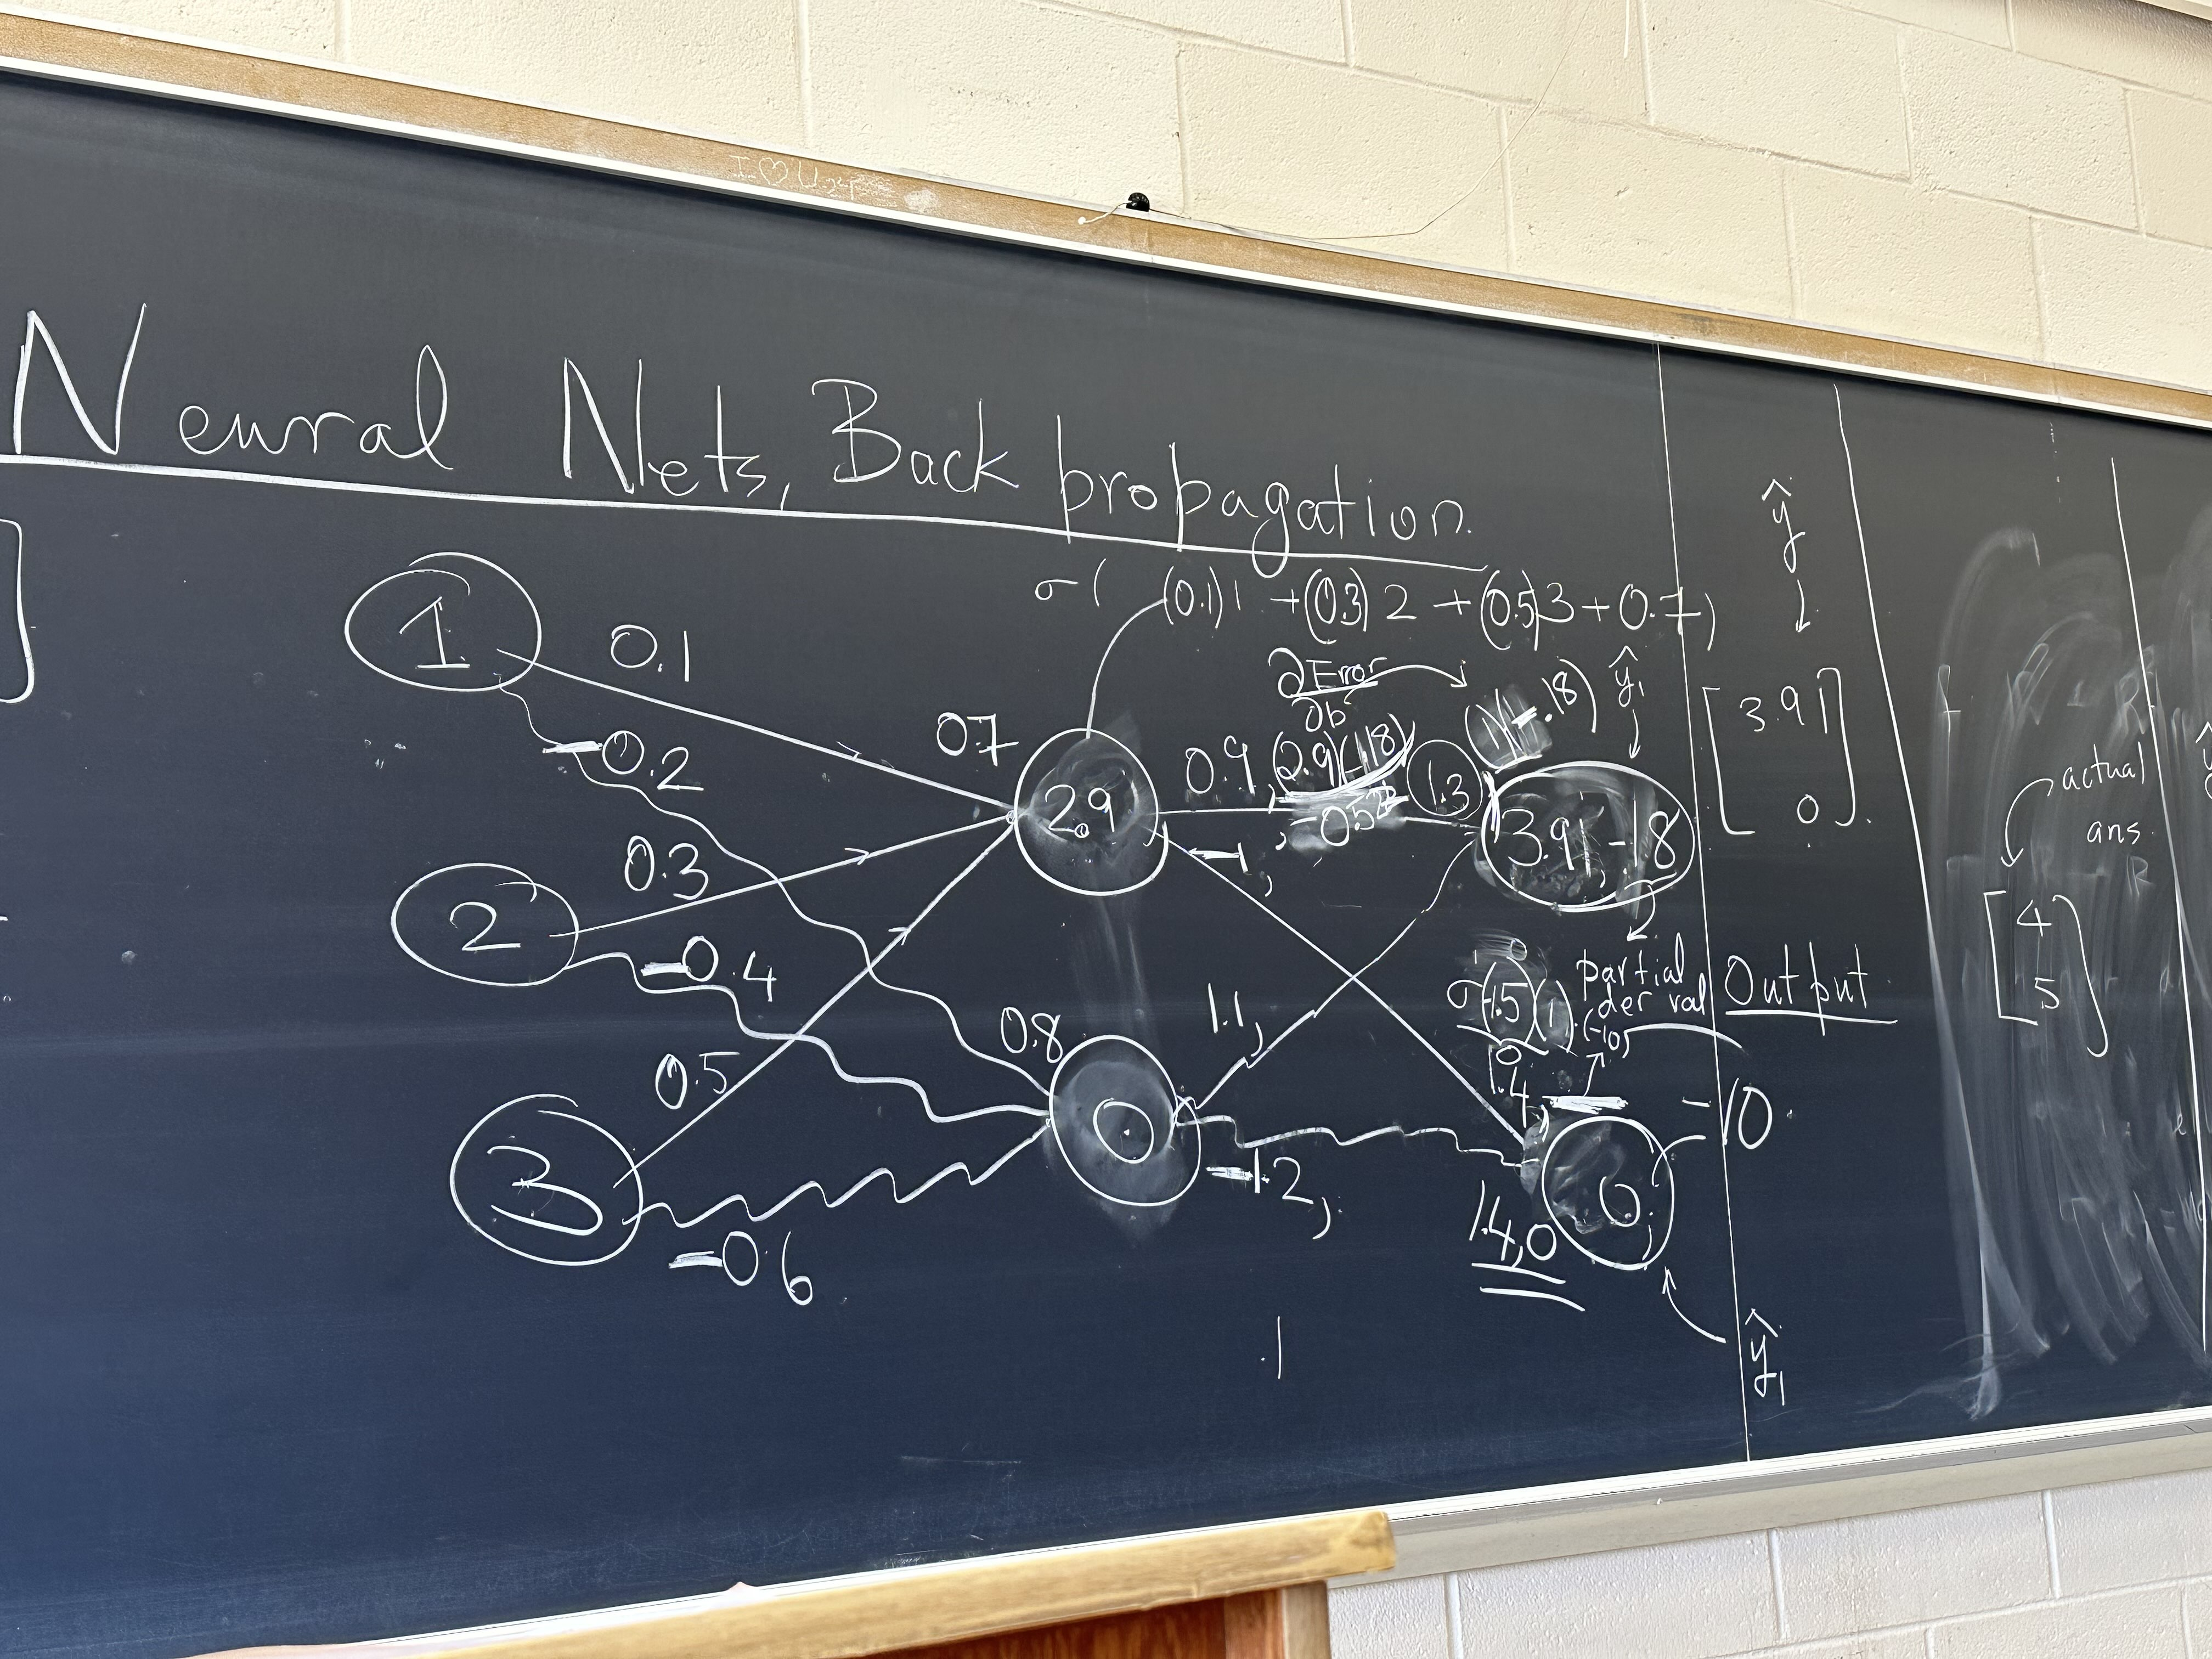
\includegraphics[width=0.5\textwidth]{NN.jpg}
        \caption{Neural Net}
        \label{fig:example_image}
    \end{figure}







\end{document}